%
%
%
% Group addresses by affiliation; use superscriptaddress for long
% author lists, or if there are many overlapping affiliations.
% For Phys. Rev. appearance, change preprint to twocolumn.
% Choose pra, prb, prc, prd, pre, prl, prstab, prstper, or rmp for journal
%  Add 'draft' option to mark overfull boxes with black boxes
%  Add 'showkeys' option to make keywords appear
\documentclass[aps,pra,reprint, onecolumn, showkeys]{revtex4-2}
%\documentclass[aps,pra,reprint]{revtex4-2}
\usepackage{lipsum}
\usepackage{listings}
\usepackage{xcolor}

\definecolor{codegreen}{rgb}{0,0.6,0}
\definecolor{codegray}{rgb}{0.5,0.5,0.5}
\definecolor{codepurple}{rgb}{0.58,0,0.82}
\definecolor{backcolour}{rgb}{0.95,0.95,0.92}

\lstdefinestyle{pystyle}{
    commentstyle=\color{codegreen},
    keywordstyle=\color{magenta},
    numberstyle=\tiny\color{codegray},
    stringstyle=\color{codepurple},
    basicstyle=\ttfamily\footnotesize,
    breakatwhitespace=false,
    breaklines=true,
    captionpos=b,
    keepspaces=true,
    numbers=left,
    numbersep=5pt,
    showspaces=false,
    showstringspaces=false,
    showtabs=false,
    tabsize=2
}
\lstset{style=pystyle}

\usepackage{booktabs}
\usepackage{siunitx}
\usepackage{adjustbox}
\usepackage{tabularx}
\newcommand\setrow[1]{\gdef\rowmac{#1}#1\ignorespaces}
\newcommand\clearrow{\global\let\rowmac\relax}
\clearrow

\newcommand{\red}[1]{\textcolor{red}{#1}}
\newcommand{\blue}[1]{\textcolor{blue}{\textbf{figure: #1}}}
\newcommand{\teal}[1]{\textcolor{teal}{\textbf{equation: #1}}}
\newcommand{\purple}[1]{\textcolor{purple}{\textbf{reference: #1}}}

\usepackage{amsmath}


\begin{document}

% Title of paper
\title{Systematic comparison between time-independent and time-dependent \\ hamiltonian approach to quantum search}

% repeat the \author .. \affiliation  etc. as needed
% \email, \thanks, \homepage, \altaffiliation all apply to the current
% author. Explanatory text should go in the []'s, actual e-mail
% address or url should go in the {}'s for \email and \homepage.
% Please use the appropriate macro foreach each type of information

% \affiliation command applies to all authors since the last
% \affiliation command. The \affiliation command should follow the
% other information
% \affiliation can be followed by \email, \homepage, \thanks as well.
\author{Matteo Garbellini}
%\email[]{matteo.garbellini@studenti.unimi.it}
%\homepage[]{Your web page}
%\thanks{}
%\altaffiliation{}
\affiliation{Department of Physics \\ Universit\`a degli Studi di Milano \\ }

%Collaboration name if desired (requires use of superscriptaddress
%option in \documentclass). \noaffiliation is required (may also be
%used with the \author command).
%\collaboration can be followed by \email, \homepage, \thanks as well.
%\collaboration{}
%\noaffiliation

\date{\today}

%\begin{abstract}
%We introduce a novel algorithm for quantum search based on an dynamical implementation of the traditional laplacian hamiltonian, taking advantages of the adiabatic theorem and its implication. We then study the worst case scenario of a simple N-dimensional ring, which gives great localization results but poor time-optimized search results. We then apply the same method to the complete graph, trying to improve the standard continous quantum-walk Grover algorithm. Different time stepping functions are investigated, hopefully giving some useful insight on the dynamic of the constructed hamiltonian.
%\end{abstract}

% insert suggested keywords - APS authors don't need to do this
\keywords{Quantum Search, Quantum Walk, Adiabatic Theorem}

%\maketitle must follow title, authors, abstract, and keywords
\maketitle

% body of paper here - Use proper section commands
% References should be done using the \cite, \ref, and \label commands

Legend: \\
\red{\textbf{Red text is comment text with general guidelines on what to write in that particular section.}}\\
\blue{Blue text is for figures and tables needed.} \\
\teal{Green text is additional equation needed.} \\
\purple{Purple text is for references.}

% % % % % % % % %
% INTRODUCTION  %
% % % % % % % % %
\section{Introduction}
This report can be summarized as follows.
\begin{itemize}
\item In Section II a review of the background topics is presented, with particular enphasis on Quantum Walks, Quantum Search and the Adiabatic Theorem. A brief introduction on Graph Theory is presented as well, in order to define the working context.
\item In Section III we discuss the Dynamics, focusing on the time dependent and time independent hamiltonian approach to quantum search, as well as the Methods, i.e. the numerical solving of schroedinger equation and more broadly the numerical evolution of the system. A brief but not less important introduction to the computational methods (e.g. optimization algorithms and solver) is presented.
\item In Section IV we present results for selected topologies, namely the \textit{worst-case-scenario} Circular Graph and the \textit{best-case-scenario} Complete Graph. For the two selected topologies we compare the known time-independent approach and the time-dependent, in particular defining two qualitative characteristics for results: optimized search and localization.
\item Section V presents a summary of the work done so far, and the further developments to be made.
\end{itemize}

%%%%%%%
%BACKGROUND
%%%%%%%
\section{Background}

\subsection{Graph Theory}
A graph G is defined as a ordered pair $(V,E)$, where V is a set of vertices and E is a set of edges, which represent the connection between any two pair of vertices. If indeed any two vertices $(i,j)$ are connected by an edge we define as adjacent, and from this we can construct the \textit{adjacency matrix} A as:
\begin{equation}
A_{ij} = \begin{cases} 1 & (i,j)\in G \\ 0 & \mbox{otherwise} \end{cases}
\end{equation}
which represents the connectivity of the graph. We can then describe the degree of each vertex of the graph, namely the number of vertices (excluding itself) connected to it, through the \textit{degree diagonal matrix} $D_{jj} = deg(j)$.\\
It is also useful to introduce the \textit{laplacian matrix} defined as
\begin{equation}
  L = A-D
\end{equation}
which we'll later see describes the quantum walk evolution.\\

Throughout this work we focus our attention on two particular graph topologies: the \textbf{circular} graph and the \textbf{complete} graph (FIG. 1).


\begin{figure}[ht]
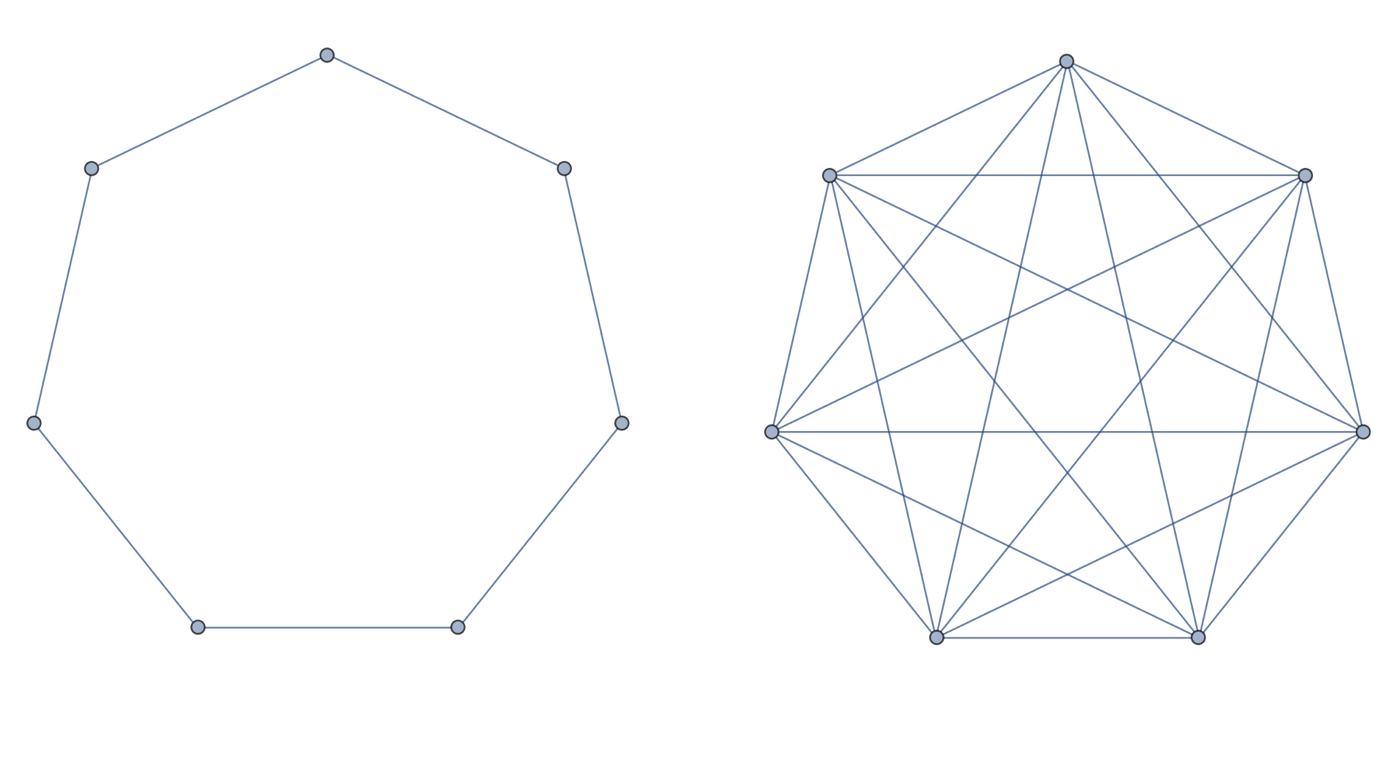
\includegraphics[width=9.5cm]{./figures/graph.png}%
\caption{Pictorial representation of a circular graph (left) and a complete graph (right) with N=7}
\end{figure}

\subsection{Quantum Walks}
The continous time quantum walk is the direct analougue of the classical random walk. Given a graph G, a random walk is a Markov process with a fixed probability for unit time $\gamma$ of jumping to an adjacent vertex $j$. This particular walk can be described by a linear differential equation in terms of probability, namely

\begin{equation}
  \frac{d}{dt}p_j(t) = \gamma\sum_{k}L_{jk}p_k(t)
\end{equation}

where $p_j(t)$ is the probability of being on the vertex $j$ at time $t$.\\
The quantum analogue takes place in an N-dimentional Hilbert space spanned by the states (vertex) $|j\rangle$ of the graph G. Instead of considering the classical probability as we previosuly did, we consider the probability time-dependent amplitudes $q_j(t) = \langle j|\psi(t)\rangle$, where $|\psi\rangle$ is a general time-dependent state. The differential equation takes thus the form of

\begin{equation}
  i\frac{d}{dt}q_j(t) = \sum_{k}H_{jk}q_k(t)
\end{equation}
The continous-time quantum walk is defined by letting $H=-\gamma L$, where $L$ is the previosuly defined Laplacian matrix.


\subsection{Quantum Search with Continous-Time Quantum Walk}
\purple{Spatial Search by Quantum Walk, \textit{A. Childs, J. Goldstone}, quant-ph/0306054v2}\\
We now address the quantum search problem firstly formulated as Grover's algorithm and then extending it to the search on a graph using quantum walks. \\
To approach the Grover problem with quantum walk it's necessary to modify the hamiltonian such that the vertex $|w\rangle$, i.e. the target, is somewhat special. Following Grover's oracle an oracle hamiltonian $H_w$ is introduced

\begin{equation}
  H_w = -|w\rangle\langle w|
\end{equation}

which in particular has energy zero for all but the vertex $|w\rangle$ for which it has enenergy $-1$. Therefore the Grover problem, i.e. quantum search, becomes finding the ground state of such hamiltonian. To do so we consider the time-independent hamiltonian of the form
\begin{equation}
  H = -\gamma L + H_w = -\gamma L -|w\rangle\langle w|
\end{equation}
where L is the laplacian of the graph, which contains the information of the dynamics over that particular graph topology. The evolution of the quantum walk is therefore governed by this hamiltonian.\\

We then begin considering the superposition of all possible state, namely
\begin{equation}
  |s\rangle = \frac{1}{\sqrt{N}}\sum_j|j\rangle
\end{equation}
and run the quantum walk for time T. The evolved state is then measured in the vertex basis. Our objective is to find the optimal value of $\gamma$ so that the success probability is as close as possible to 1 for the smallest T

\begin{equation}
 c
\end{equation}
where $\psi(T)$ is the evolved superposition state $|s\rangle$


\subsection{Adiabatic Theorem}
\purple{Quantum Computation by Adiabatic Evolution \textit{E. Farhi, J. Goldstone, S. Gutmann, M. Sipser}, quant-ph/0001106 }\\


A quantum system evolves according to the Schroedinger equation
\begin{equation}
	i\frac{d}{dt}|\psi(t)\rangle = H(t)|\psi(t)\rangle
\end{equation}
and defining the instantaneous eigenstates and eigenvalues of H(t) by
\begin{equation}
	H(t)|l;t\rangle = E_l(t)|l;t\rangle
\end{equation}
such that $E_0(t) \geq E_1(t) \geq ... \geq E_{N-1}(t)$. \\
The adiabatic theorem states that if the gap between the two lowest energy levels, $E_{1}(t) - E_{0}(t) > 0$, is stritcly greater than zero then for $T\rightarrow \infty$ the probability of being in the ground state is equal to one, namely
\begin{equation}
	\lim_{T \to \infty} |\langle l=0;t = T | \psi(T)\rangle| = 1
\end{equation}
This means that if the system is chosen to evolve at a slow enough rate, the instantaneous hamiltonian will remain in the ground state throught the evolution. It is useful to consider a smooth one-parameter hamiltonian $H(s)$ such that $s=t/T$, with $t \in [0,T]$ so that $s \in [0,1]$.
Let's now define the energy minimum gap by
\begin{equation}
	g_{min} = \min_{0 \leq s \leq 1} (E_1(s)-E_0(s))
\end{equation}
In addition we can find a time lower bound $T^*$ such that for $T\gg T^{*}$ the probability is arbitrarily close to 1, in detail
\begin{equation}
	T \gg \frac{\varepsilon}{g^{2}_{min}}
\end{equation}
where
\begin{equation}
	\varepsilon = \max_{0 \leq s \leq 1} \Big| \Big\langle l=1;s\Big| \frac{dH(s)}{dt} \Big| l=0;s\Big\rangle\Big|
\end{equation}

Let's now discuss how to take advantage of the adiabatic theorem introducting the usual way in which the adiabatic evolution is implemented. It is often presented a problem hamiltonian $H_P$ whose ground state is not so straight forward to find; on the other hand we can prepare the system in abeginning hamiltonian $H_B$ whose ground state is known. The problem hamiltonian encodes the solution of the problem, while the beginning hamiltonian is a tool for easily preparing the state to be evolved. The adiabatic implementation then consists, assuming that the ground state of $H_P$ is unique, in having a time dependent hamiltonian $H(s)$ such that
\begin{equation}
	H(s) = (1-s)H_B + s H_P
\end{equation}
In this way we can prepare for $s=0$ the system in $H_B$ and let it evolve so that for $s=1$ it reaches $H_P$. Thanks to the adiabatic theorem, if it's made to evolve sufficiently slowly we will find ourself in the ground state of the problem hamiltonian, which is exactly the solution.


%%%%%%%
%DYNAMICS AND METHODS
%%%%%%%
\section{Dynamics and Methods}
In this section we look more in depth at the time-independent and time-dependent hamiltonian used for the search algorithm, putting particular focus on the time function that regulates the evolution of the hamiltonian. We then explore the possible way to numerically solve the schroedinger equation, giving reasoning of why we decided to solve it numerically using a Runge-Kutta integrator. Last but not least we look at the computational methods, namely the code written and the optimization and integrator algorithms used.

\subsection{Time Independent Hamiltonian}
As we've seen in Section ?, the quantum search with quantum walk consists in finding the probability $p = |\langle w|\psi(T)\rangle|^2$, thus we're interested in the evolution of the beginnig state $|s\rangle$ using the hamiltonian:
\begin{equation}
H = -L -\gamma|w\rangle\langle w|
\end{equation}
that differs from the hamiltonian introduced by Goldstone \& Childs having the $\gamma$ term in front of the oracle instead of the laplacian. The two, however, describe the same evolution (apart from a global phase). \\
The evolution of a state for the time independent hamiltonian is given by the operator S(t)
%\begin{equation*}
%\begin{split}
%  p & = |\langle w|\psi(t)\rangle|^2  \\ & =  |\langle w|S(t)|s\rangle|^2 \\ & = |\langle w|e^{-\frac{i}{\hbar}Ht}|s\rangle|^2 \\
%  & = |\langle w|e^{-\frac{i}{\hbar}\gamma(-\frac{1}{\gamma}-|w\rangle\langle w|)t}|s\rangle|^2
%\end{split}
%\end{equation*}

\begin{equation}
  U(t) = e^{-\frac{i}{\hbar}Ht}
\end{equation}
Therefore the probability is given by the following
\begin{equation*}
\begin{split}
  p & = |\langle w|\psi(t)\rangle|^2  \\ & = |\langle w|U(t)|s\rangle| ^2 \\& =|\langle w|e^{-\frac{i}{\hbar}Ht}|s\rangle|^2
\end{split}
\end{equation*}
From a computational point of view this evolution is a simple matrix multiplication, and doesn not require any particular tool.

\subsection{Time Dependent Hamiltonian}
We introduce a time dependent hamiltonian that follows from the adiabatic implementation discussed in Section ? and the time-independent approach previously discussed. The intuition behind this implementation comes from the idea of \textit{adiabatically} turn on the oracle hamiltonian. Theoretically this should give us the advantage discussed in (Section II - Adiabatic Theorem), namely the high probability of finding the solution with the possible expense of longer time scaling. \\
The hamiltonian is thus in the form of
\begin{equation}
H(t) = (1-s(t))L + \gamma s(t)|w\rangle\langle w|
\end{equation}
where $s(t)$ is a function of time that will be later discussed in more detail. \\

The probability is calculated similarly to the time-independent hamiltonian, with the exception that the time evolution operator is given by

\begin{equation}
U(t) = \mbox{exp} \Big\{ -\frac{i}{\hbar} \int_{0}^{t}dt'H(t') \Big\}
\end{equation}
This makes finding the evolved state $|\psi(t)\rangle$ not so straight-forward, in particular for the circular graph for which the hamiltonian does not show any particular pattern/property. A few approximation could be used for this task such as the \textit{Dyson Series} and the \textit{Magnus Expansion}. However, for our specific scenario, for which we only needed the evolved state we decided to opt for \textit{solving the Schroedinger equation}, namely

\begin{equation}
  i\frac{d}{dt}|\psi(t)\rangle = H |\psi(t)\rangle
\end{equation}
Since H is a matrix we had to solve it for components. Recalling that $|\psi\rangle$ is a vector in an N-dimensional Hilbert space, we need to solve N-differential equations of the form:

\begin{equation}
\frac{d}{dt}|\psi_i(t)\rangle = \sum_jH_{ij}|\psi_i(t)\rangle
\end{equation}

Once the N solutions are found, the probability is easily found with $p=|\langle w |\psi(t)\rangle|^2$. It's worth noting that some additional normalization on the found solution might be necessary due to the integrator used, however a more in depth discussion on the integrator and normalization can be found in the Appendix.


\subsection{Comments on the form of s(t)}
\red{Discussion on the time-stepping function $s(t)$ (or better  $g_T(t)$). Why did we choose this particular shape for the function? Are we expecting any improvements? \\ In particular if we follow what has been said by Cerf et al. the function should be steeper (evolving faster) when the separation $E_1(t)-E_0(t)$ is larger, and slower for small separation. Looking at the separation distribution the functions used (sqrt, cbrt, linear) do not fit to this model. \\ It's interesting to show, probably in the Results section rathen than here, how significant is the shape of s(t) in the final probability}


\subsection{Computational Routines}
Throught the analysis the goal was to find the optimal probability for the specific scenario, and the procedure varied depending on the graph topology and the hamiltonian considered. That being said, we can characterize them as follows:
\begin{itemize}
  \item \textbf{$\beta$ and T probability optimization:} as it might imply, we run an optimization using $\beta$ and time as parameters, trying to maximize the probability. This process is quite computationally intensive, so except for the time-independent algorithm we employ the following two technique.
  \item \textbf{T optimization for fixed $\beta$:} this technique is quite useful when we are only qualitatively interested at the probability distribution. Thus sampling a fix number of $beta$ and optimizing on the time variable. This results in a great computational time improvement, particularly for the time-dependent approach.
  \item \textbf{probability grid evaluation:} this technique consists in sampling both time and $\beta$ and evaluating the probability for all the time-beta combinations, namely evaluating the probability on a grid. The advantage of such approach is the much less computational time needed since a single evaluation is much faster than an optimization \blue{might be interesting having a graph comparing computational time}. Secondly true optimization tries to find the absolute maxima, to the expence of having a larger T (remember, we're trying to find the highest probability for the shortest time). As an example, we might find a probability p=0.95 for T = 10 using the grid evaluation, although the true maximum is p=0.96 for T = 35. Is indeed clear that the 0.01 in greater probability does not balances the disadvatange of more than double time.
\end{itemize}
Additional information on the optimization algorithms used can be found in the Appendix.

\clearpage
%%%%%%%
%RESULTS FOR SELECTED
%TOPOLOGIES
%%%%%%%
\section{Results for selected topologies}

\subsection{Search vs Localization}
We shall describe the possible outcomes of the previously introduced hamiltonian and characterize them as \textbf{localization} and \textbf{optimized search}. The first describes the finding with high probability of the solution without particular interest in the time needed to reach that particular solution. For example, as we shall see later in Section V, the ring-graph is known for not working with traditional quantum-walk algorithm (i.e. found with low probability), but thanks to the adiabatic nature for $T \to \infty$ the solution is found with probability 1. \\

On the other hand we know that for our algorithm to be somewhat interesting from the perspective of the quantum search we need at least the same speedup we get from the traditional quantum-walk Grover, namely $O(\sqrt(N))$. We're thus optimizing for maximum probability and minimum time; in addition as we shall see later we'll also consider the possibility of repeating the search an $n$ amount of times, and get a less than optimal search for each iteration but better time (sum of time, actually) overall. It is indeed this what we call \textit{optimized search}.


\subsection{Circular graph}
\subsubsection{Time-Independent Benchmarks}
The first step in our analysis is to compute some benchmark for the time-independent hamiltonian, in order to later compare the time-dependent approach. This is particularly interesting since we know that th quantum search time-independent algorithm does not work with the circular graph, namely the found probability is periodical and for large N converges to p = 0.1.\\ \blue{Converging probability to 0.1 for large N}\\

Using the time-independent hamiltonian introduced before we optimized the probability on T and $\beta$ for circular graphs up to N=31. It is worth noting that we considered only odd graphs, since it made an easier center-placement of the oracle site state. The following are the results:\\
\blue{time-independent benchmarks up to N=31}\\

\begin{figure}[ht]
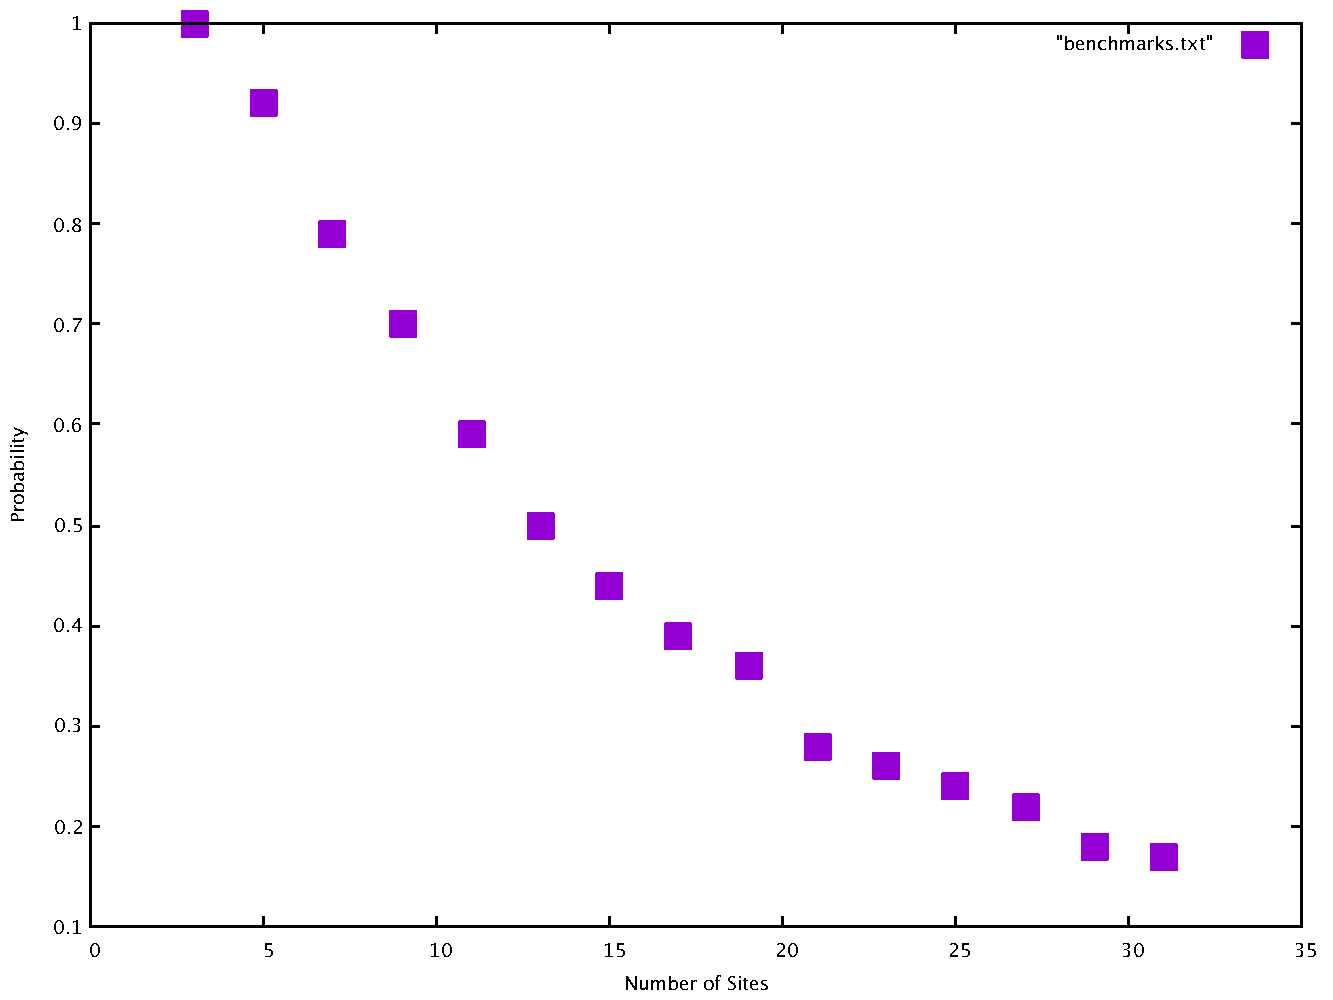
\includegraphics[width=10cm]{./figures/benchmarks.pdf}%
\caption{Time Independent Benchmarks up to N=31}
\end{figure}

It is clear that the time-independent algorithm does indeed not work, as we expected. The probability decreases as the number of sites N increases, \red{converging for large N to $p=0.1$}.

\subsubsection{Time-Dependent Algorithm}
We then considered the time-dependent hamiltonian introduced in Section ?, and following the \textit{probability grid evaluation} procedure discussed before we computed the probability. Given the computational efficency over the regular $\beta$-T optimization we were able to compute results up to N = 71, although from 31 to 71 only the 1st and 7th (e.g. 41,47) were calculated. \\

It is however clear that the grid-evaluation approach does not produce unique values of $(T,\beta)$ corrisponding to the absolute probability maximum. On the other hand is able to give a qualitative idea on the probability distribution for various $(T,\beta)$ combinations. We then present the found data with a \textbf{heatmap plot} such the one below, which makes quite easy to visualize the result.\\ \blue{heatmap plot example}\\

\begin{figure}[ht]
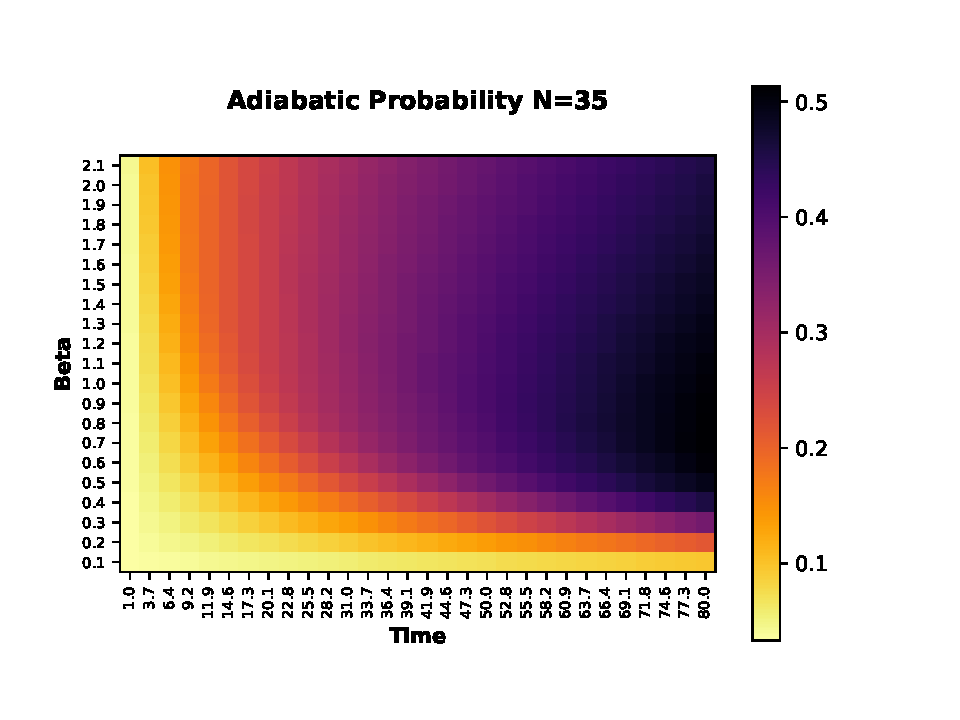
\includegraphics[width=10cm]{./figures/example.pdf}%
\caption{Time Dependent heatmap example, N=35}
\end{figure}

The task now is two develop a method to compare the time-independent and time-dependent algorithms. We first naively look at a qualitative comparison that immediately shows that the time-dependent algorithm is able to find higher probabilities but at the expense of worst time scaling; secondly we introduce a quantity to compare the two methods numerically.

\subsubsection{Qualitative Comparison}
In order to qualitatively compare the two approaches to quantum search we will consider a heatmap plot where we superimpose probability \textbf{contour lines} corrisponding to the following probability (and with the following format):
\begin{itemize}
  \item (solid) p = 0.99, p = 0.95, p = 0.90 for the time-dependent results
  \item (dashed) the probability found in the corrisponding time-independent results
  \item (dashed) double the probability (as long as it doesn't exceed unity) found for the time-independent
 result
\end{itemize}
These, with the corrisponding time T at which the time-independent probability is found (given by a vertical line), should give a qualitative method to compare the two approaches, namely looking at the intersection between the first dashed line and the vertical time-line.\\


\begin{figure}
\begin{tabular}{cc}
  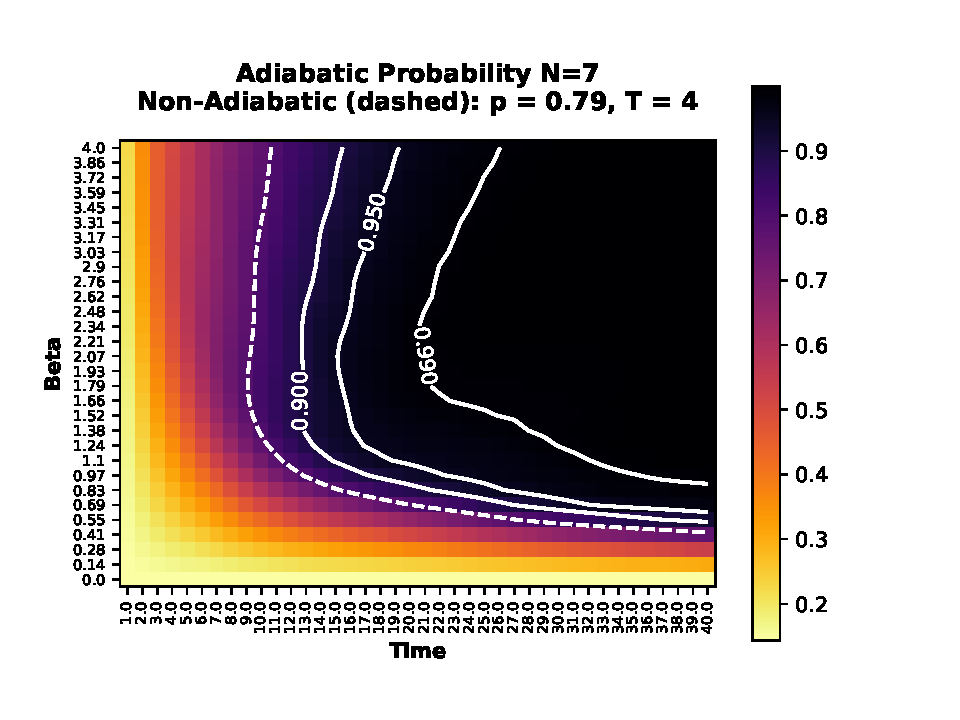
\includegraphics[width=90mm]{./figures/7_probability_heatmap.pdf} &   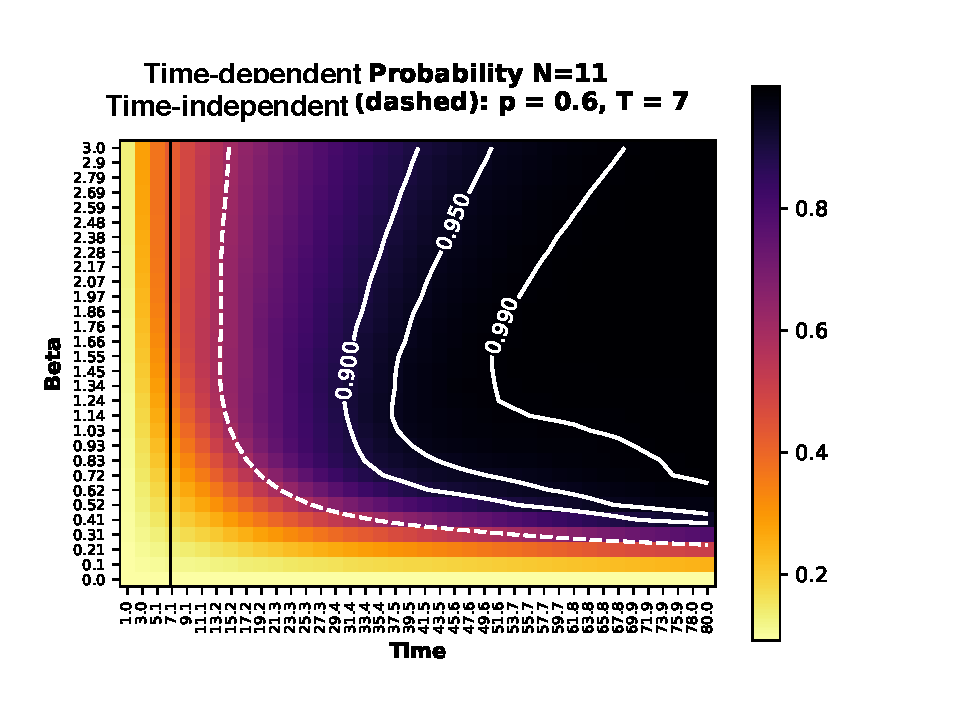
\includegraphics[width=90mm]{./figures/11_probability_heatmap.pdf} \\
(a) N = 7 & (b) N = 11\\[6pt]
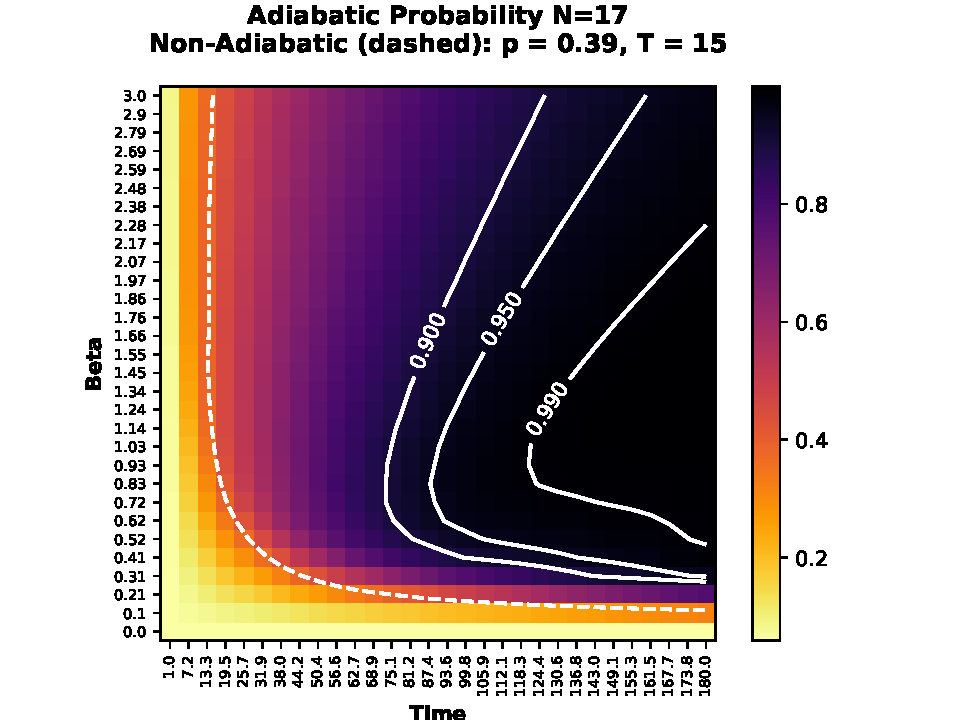
\includegraphics[width=90mm]{./figures/17_probability_heatmap.pdf} &   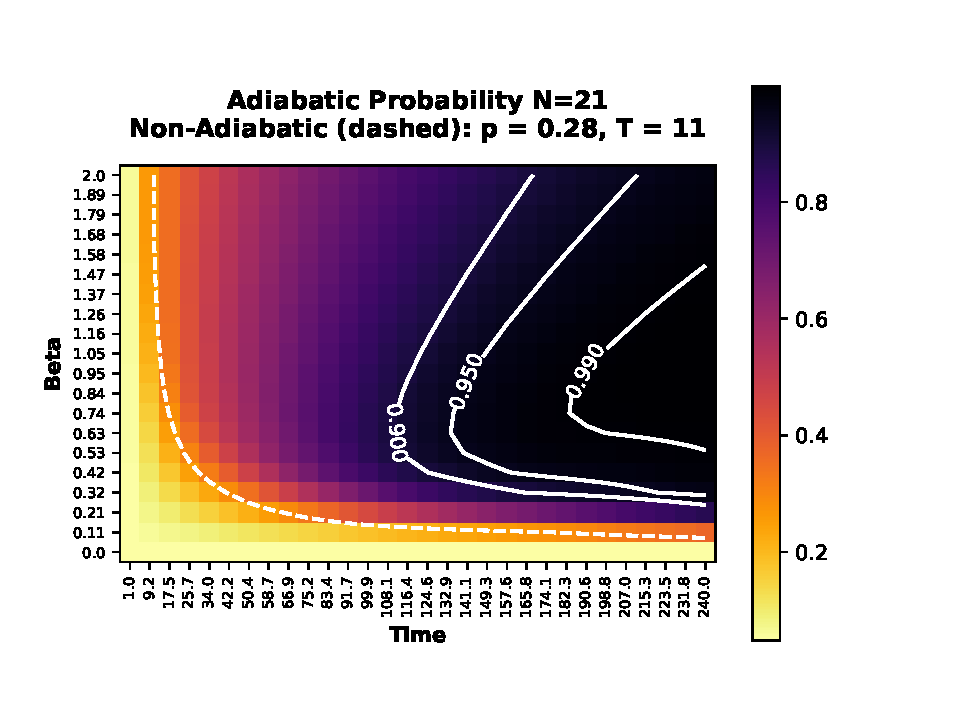
\includegraphics[width=90mm]{./figures/21_probability_heatmap.pdf} \\
(a) N = 17 & (b) N = 21\\[6pt]
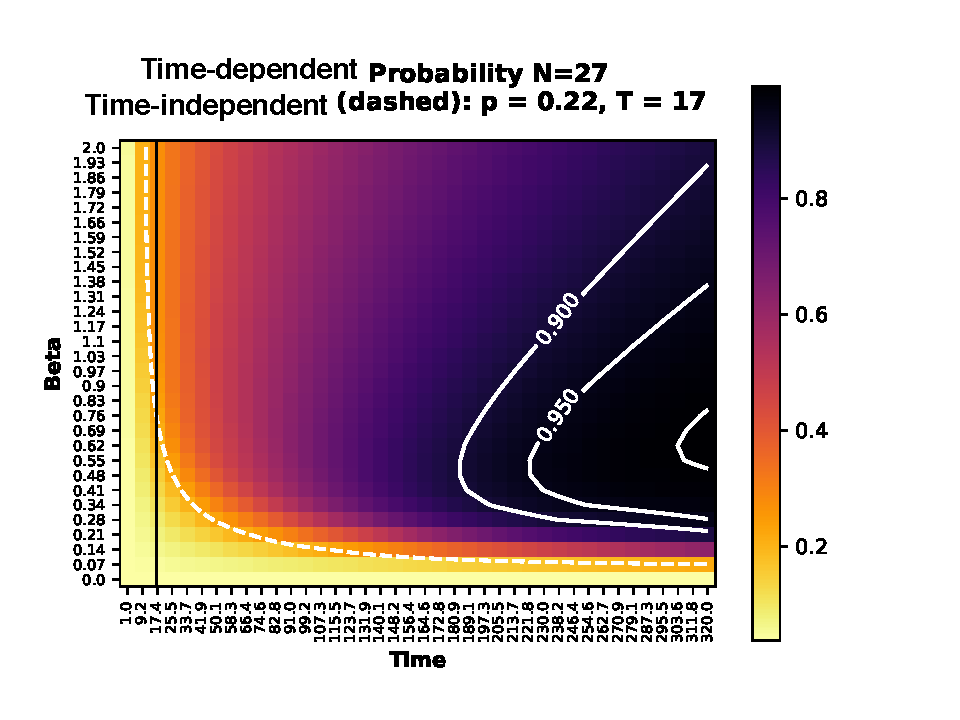
\includegraphics[width=90mm]{./figures/27_probability_heatmap.pdf} &   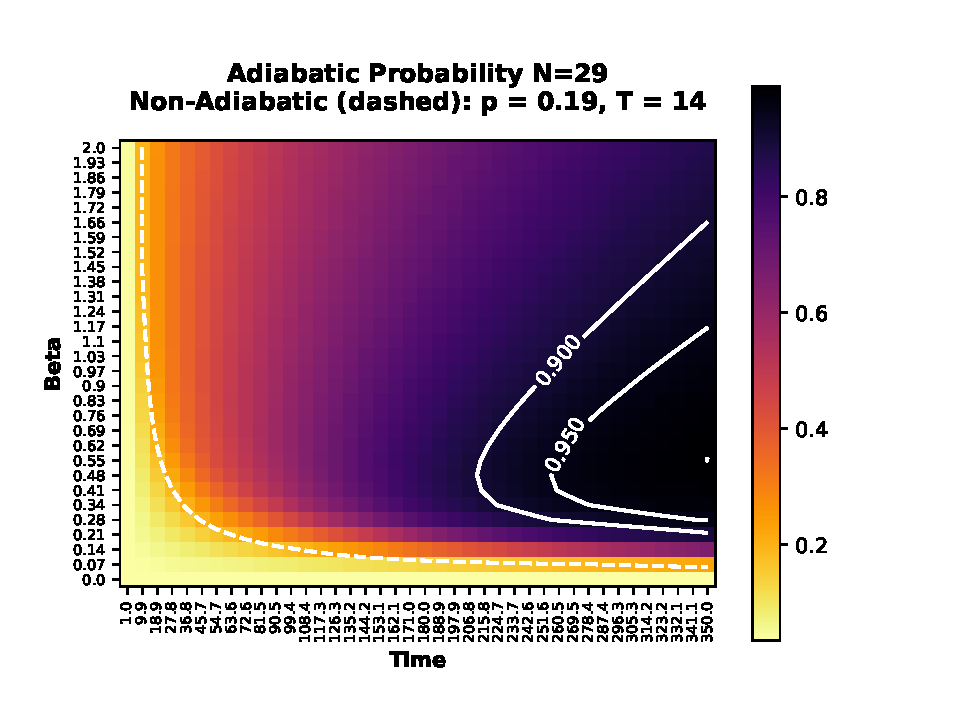
\includegraphics[width=90mm]{./figures/29_probability_heatmap.pdf} \\
(a) N = 27 & (b) N = 29\\[6pt]
\end{tabular}
\end{figure}

%\clearpage

\subsubsection{Numerical Comparison}
In order to numerically compare the two approaches we define a quantity $\delta$ in the following way:
\begin{equation}
  \delta = \min\Big(\frac{T}{p}\Big)
\end{equation}
The quantity T/p represents the total time necessary to get to unitary probability. Finding the minimum of that quantity corresponds to finding the best combination of T and p that gets to unity with the minimum T. \\

What we do is thus for each vertical column of the grid, i.e. constant T and variable $\beta$, computing the maximum probability and finding the quantity T/p. We than find the minimum of all the T/p calculated. In this way we \textbf{reduce a grid to a single value} to compare to the time-independent results. \\

The following plot compares the time-independent approach to the time-dependent one, using for the first the quantity T/p evaluated with the \textit{$\beta$-T optimized} probability while the latter uses the quantity $\delta$. \\

\begin{figure}[ht]
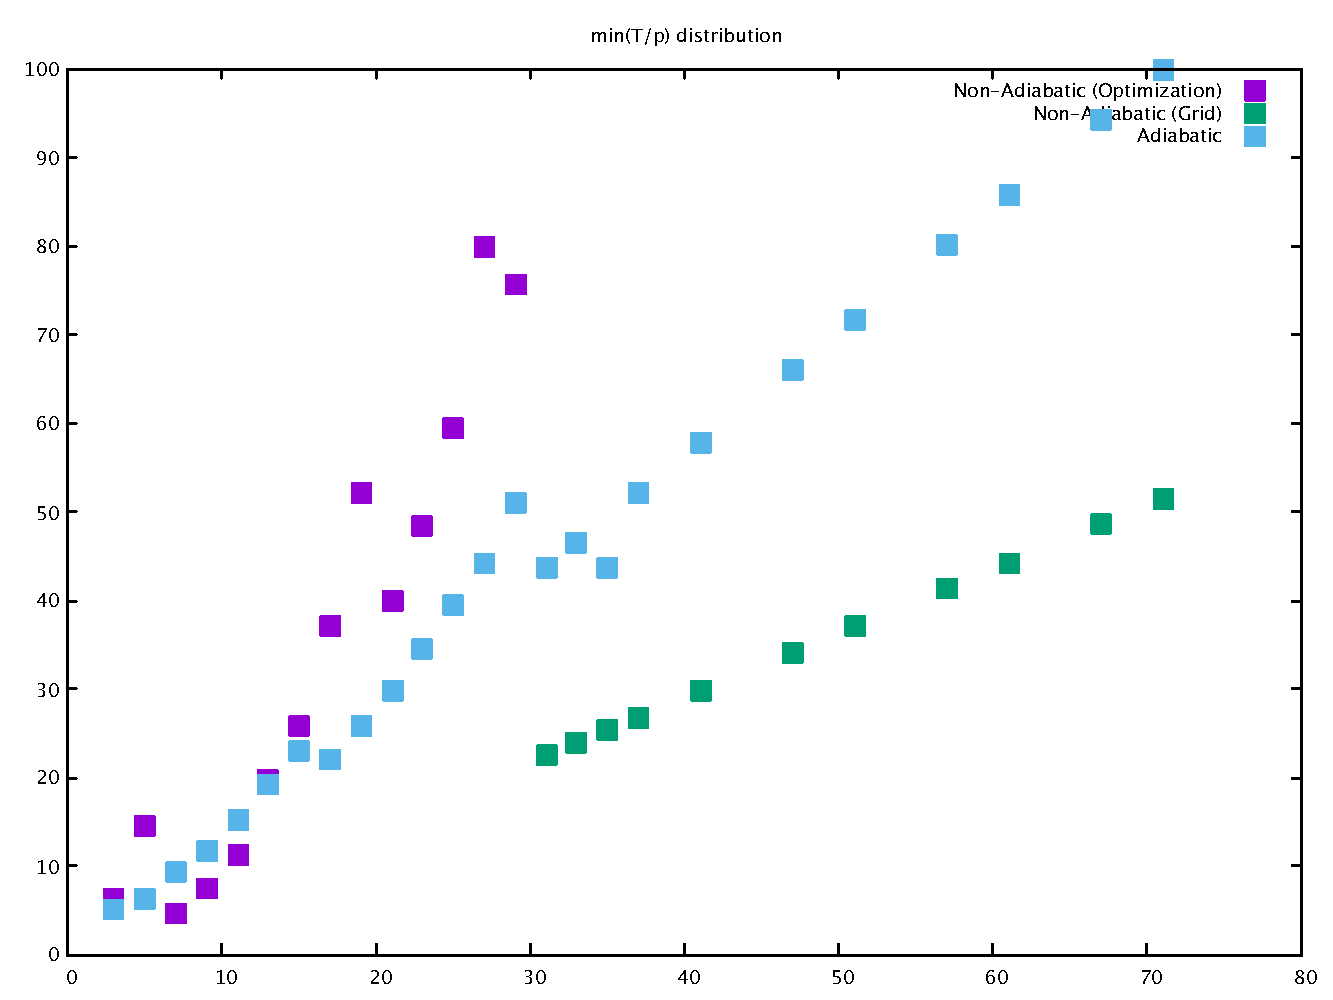
\includegraphics[width=10cm]{./figures/delta.pdf}%
\caption{delta values comparing methods}
\end{figure}


\subsubsection{Different s(t) shapes}
As we introduced in Section ? we're interested in determining how influencial is the shape of s(t) in the probability distribution. We then proceed as in Section ? using the step function s(t) previously discussed. \\ To compare we consider the quantity $\delta$. Since we're interested in the trend for large N we ignore small N and only consider a few sampled N between 35-70.

\clearpage
\begin{figure}[ht]
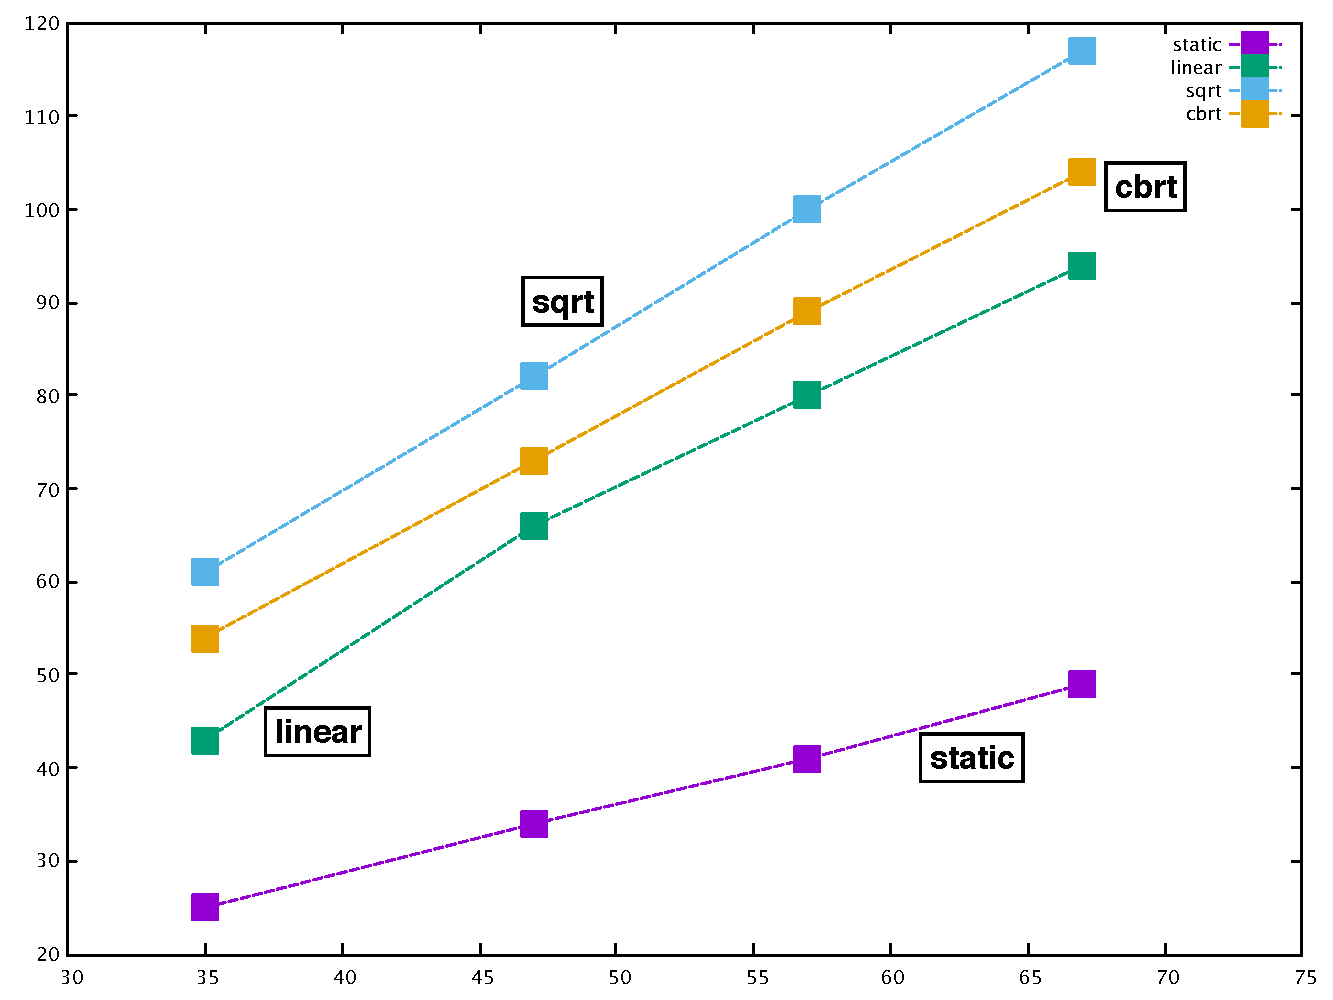
\includegraphics[width=10cm]{./figures/9_Giugno.pdf}
\caption{Delta distrubution for different s(t). Computed for N = 35,47,57,67}
\end{figure}

As the plot shows however we do not see any speedup for functions that are not linear, on the contrary we do get poorer results. The time-independent implementation remains the best performing one, followed by linear, cubic root and square root. \red{I wonder whether this approach was well-thought in the first place. As was already mentioned in Section ? we might want to consider what was mentioned by Cerf et al.}

\subsubsection{Localization}
We can clearly see from the heatmap plots that we showed for the qualitative comparison that for large T the probabability gets bigger, and it's quite close to one for very large T, namely $T>10N$. A further analysis is due, focusing on studying the probability distribution. \red{Although it's clear from the adiabatic theorem and from the results that we currenly have that localization is a key feature of the time-dependent hamiltonian approach, further numerical simulations are necessary. In particular we might be interested in finding a trend (in terms of N) for few sampled probabilities, e.g. p = 0.5,0.75,0.8, 0.9, 0.95, 1  }

\subsection{Complete graph}
\red{This section should include a comparison between time dependent and time independent approach to quantum search for the complete graph. Since this topology is solvable analitically I wonder what kind of results should I put in this section.\\ It might be interesting looking into the order of the probability for p=0.9. Analytically the solution is looked for p=1, possibily (for localization in particular) we could get some speed up over $\sqrt{N}$ for probabilities less than 1. This might work particularly well if the probability is not linear in the vicinity of $\sqrt{N}$ }\\ \blue{Probability distribution for fixed $\gamma$ with increasing time}

%%%%%%%
%APPENDIX
%%%%%%%
\clearpage
\section{Appendix}
In this section an overview of the computational methods is presented, focusing the attention on specific matters: \textit{Optimization Algorithm} used for determining the optimal $\gamma$-configuration for maximum probability, \textit{Schroedinger Solver} for the time dependent hamiltonian evolution and some additional parameters for the optimal \textit{Runge-Kutta Normalization Error}. Lastly computational reasoning for the \textit{2D - Probability Heatmap} are presented. \\

Most all numerical simulations were performed using \textbf{Python} being easy and flexible to sudden changes. Numerical methods such as optimization and ODE Solver come directly from python's native \textbf{Scipy}. In addition, a CPU-multiprocessing library, \textbf{Ray}, has been used to speed up the grid probability evaluation quite noticeably. 2D - Heatmap plots were created using python matplotlib, while additional plots were created with gnuplot.

\subsection{Optimization Algorithm}
In Section II a series of benchmark were performed to compare the standard Quantum-Walk algorithm to the Adiabatic-Quantum-Walk implementation (later simply named \textit{dynamic}). In order to determine which optimization algorithm fitted the best for the task, a number of possible algorithm were tested, such as \textit{shgo, dualannealing, minimize, LHSBH} and \textit{Basin-Hopping}. \\

Due to the oscillating nature of the probability (cfr figure) the scipy native \textbf{Basinhopping algorithm} was used. As the name suggests the algorithm performs a series of randomized hops, i.e. jumps, of the coordinates in order to find the true maximum (actually, the true \textit{minimum}). This fits particularly well with the series of maxima and minima of the probability function (for fixed $\gamma$) in the static algorithm (std QWAlgorithm). Snippets of the parameters used follow.

\begin{lstlisting}[xleftmargin=0cm]
	from scipy.optimize import basinhopping
	optimization = optimize.basinhopping()
	print(optimization)
\end{lstlisting}

\subsection{Schroedinger Solver}
In Section III we presented an evolution which is governed by a time-dependent hamiltonian, used to find the evolved state $|\psi(t)\rangle$. This is accomplished by solving the usual Schroedinger equation using Scipy's \textbf{integrate.solve\_ivp}, that provides a wide varieties of integrations methods. \\

As it's routine we used Runge-Kutta RK45, which as stated in the documentation it's a explicit Runge Kutta method of order 4(5). The error is controlled assuming fourth order accuracy, but steps are taken using the fifth-order accurate formula. In addition, the integrator is adaptive, meaning that the time step is chosen for optimal error control. Regarding the error, the algorithm provides two distinct parameters to set a targeted limit, namely the \textbf{relative (rtol)} and \textbf{absolute tolerances (atol)}. The first provides a relative accuracy, i.e. the number of digits, while the latter is used to keep the local error estimate below the threshold \textit{atol + rtol*abs(y)}. Determining the correct combinations of the two parameters is key for achieving the desired error. A few of those are presented in the following table, where a worst case scenario is used and the error is evaluated on the expected normalized state. \\

\begin{center}
\begin{adjustbox}{width=6cm}
\begin{tabular}{>{\rowmac}c>{\rowmac}c>{\rowmac}c>{\rowmac}c>{\rowmac}c<{\clearrow}} \toprule
    {rtol} & {atol} & {norm} &{error} & {comp time (s)}\\ \midrule
    e-3  & e-5 & 1.0851 & -0.0851 & 83.8\\
    \setrow{\bfseries} e-3  & e-6 & 1.0198 & -0.0198 & 19.5\\
    e-3  & e-7 & 1.0188 & -0.0188 & 19.4\\
    e-3  & e-8 & 1.0187 & -0.0187 & 19.5\\ \midrule

    e-4  & e-5 & 0.9988 & 1.16e-3 & 90.6\\
    e-4  & e-6 & 0.9996 & 3.98e-4 & 21.7\\
    e-4  & e-7 & 0.9996 & 4.13e-4 & 21.4 \\
    e-4  & e-8 & 0.9996 & 4.04e-4 & 21.5 \\ \midrule

    e-5  & e-5 & 0.9989 & 1.09e-3 & 82.8\\
    e-5  & e-6 & 0.9998 & 1.81e-4 & 20.5\\
    e-5  & e-7 & 0.9999 & 1.33e-4 & 20.6\\
    e-5  & e-8 & 0.9999 & 1.21e-4 & 20.8\\ \midrule

    e-6  & e-5 & 0.9998 & 2.48e-4 & 92  \\
    e-6  & e-6 & 0.9999 & 5.78e-5 & 22.6\\
    e-6  & e-7 & 0.9999 & 2.47e-5 & 23.2\\
    e-6  & e-8 & 0.9999 & 1.68e-5 & 23.2\\ \bottomrule

\end{tabular}
\end{adjustbox}
\end{center}


\subsection{Comments on heatmap and computational time}


\subsection{Runge-Kutta normalization errors and parameters}



\end{document}
